\documentclass[12pt,letterpaper]{article}
\usepackage{graphicx}
\usepackage{scrextend}
\usepackage{vmargin}
\usepackage[utf8]{inputenc}
\usepackage[spanish]{babel}
\usepackage{subcaption}
\usepackage{caption}
\usepackage{multicol}
\usepackage{hyperref}
\usepackage{amsmath, amsthm, amssymb, amsfonts}
\usepackage[usenames]{color}
\usepackage{float}
\parindent=0mm
\pagestyle{empty}
\definecolor{citecolor}{rgb}{.12,.54,.11}
\definecolor{urlcolor}{RGB}{64, 145, 108}
\definecolor{1ee592}{RGB}{30,229,146}
\definecolor{1bac70}{RGB}{27,172,112}
\definecolor{f38638}{RGB}{243,134,56}
\definecolor{black}{RGB}{0,0,0}
\definecolor{gray}{RGB}{156,156,156}
\hypersetup{
    colorlinks=true,
    linkcolor=blue,
    filecolor=magenta,      
    urlcolor=urlcolor,
    citecolor=citecolor,
}
\begin{document}
\setmargins{2.5cm}      
{1.5cm}                     
{2cm}  
{24cm}                    
{10pt}                          
{1cm}                          
{0pt}                             
{2cm}
\subsection*{Análisis basado en imágenes de Google Earth en el periodo 25/May/2006 - 10/Ago/2019}
\begin{enumerate}
    \item Entre el 22/May/2007 - 18/May/2011 se creó un camino (ver parte superior izquierda) al noroeste del punto marcado como el Ejido "Las Abejas", con latitud y longitud [26° 1'53.60"N, 100°16'39.50"O]. Este camino fue desvaneciéndose a partir del año 2016, poco a poco hasta 2019. El camino principal desemboca en el punto amarillo, marcado para el Ejido Las Abejas, siempre mostró un color muy claro. Esto podría significar un tránsito frecuente en todo el periodo.
    \begin{figure}[H]
        \centering
        \begin{subfigure}{3.5\textwidth}
            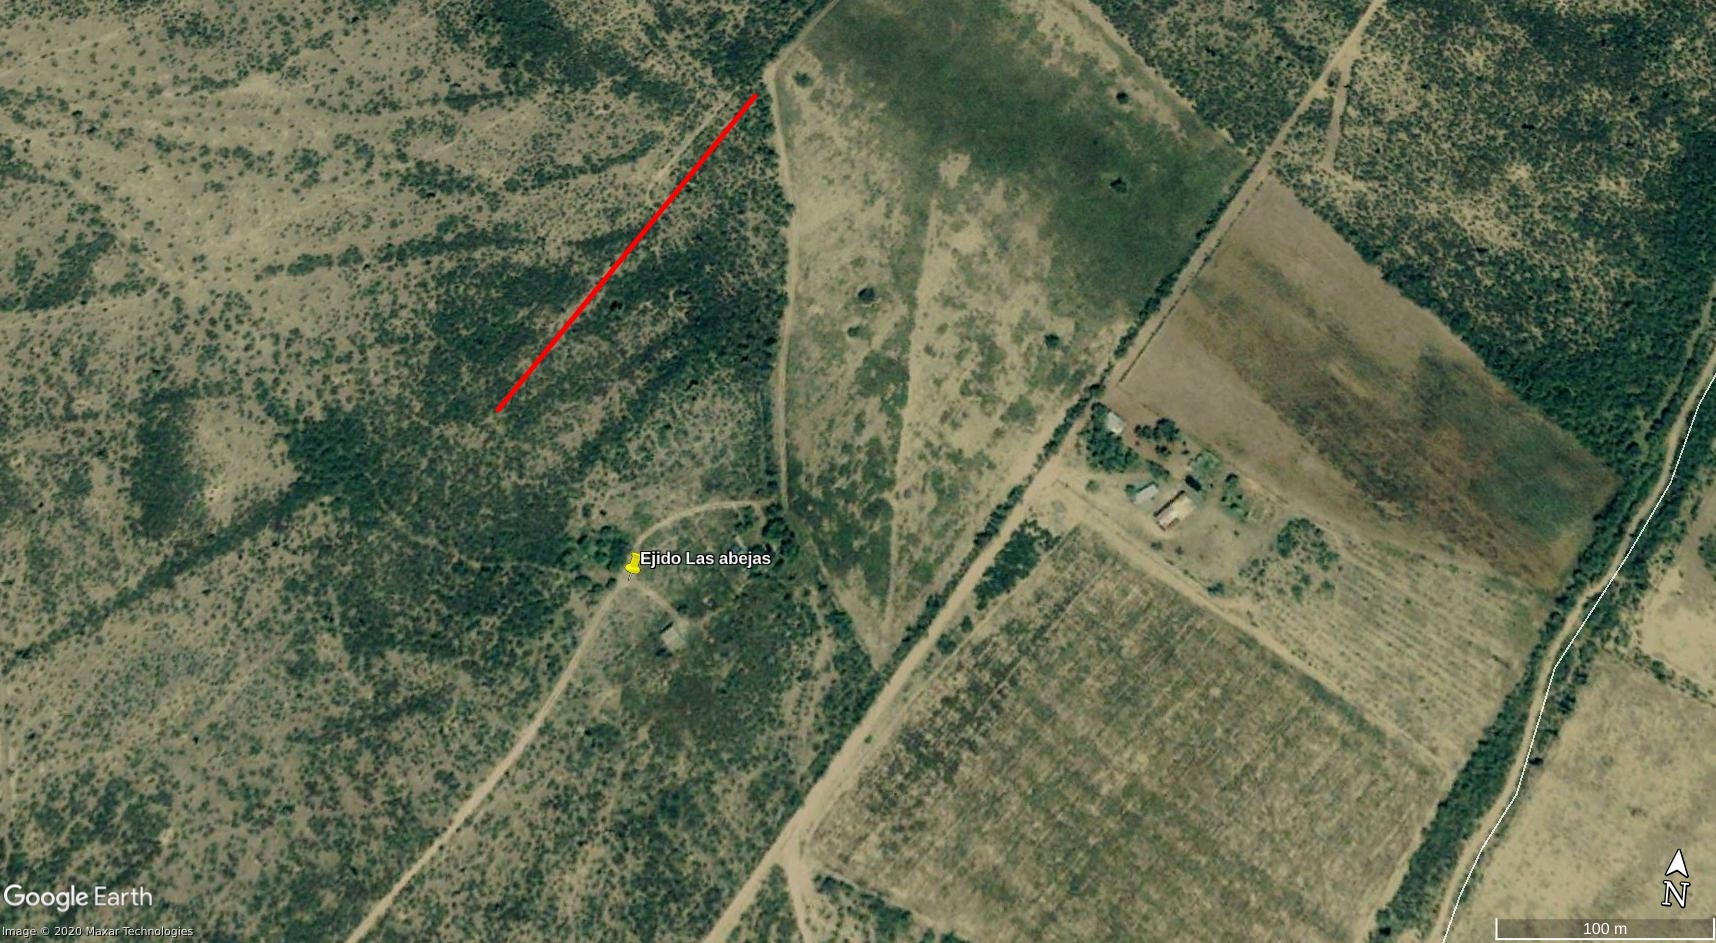
\includegraphics[scale=0.155]{070522r.jpg}
            \caption{Día 22/May/2007: sin camino}
        \end{subfigure}
        \begin{subfigure}{3.5\textwidth}
            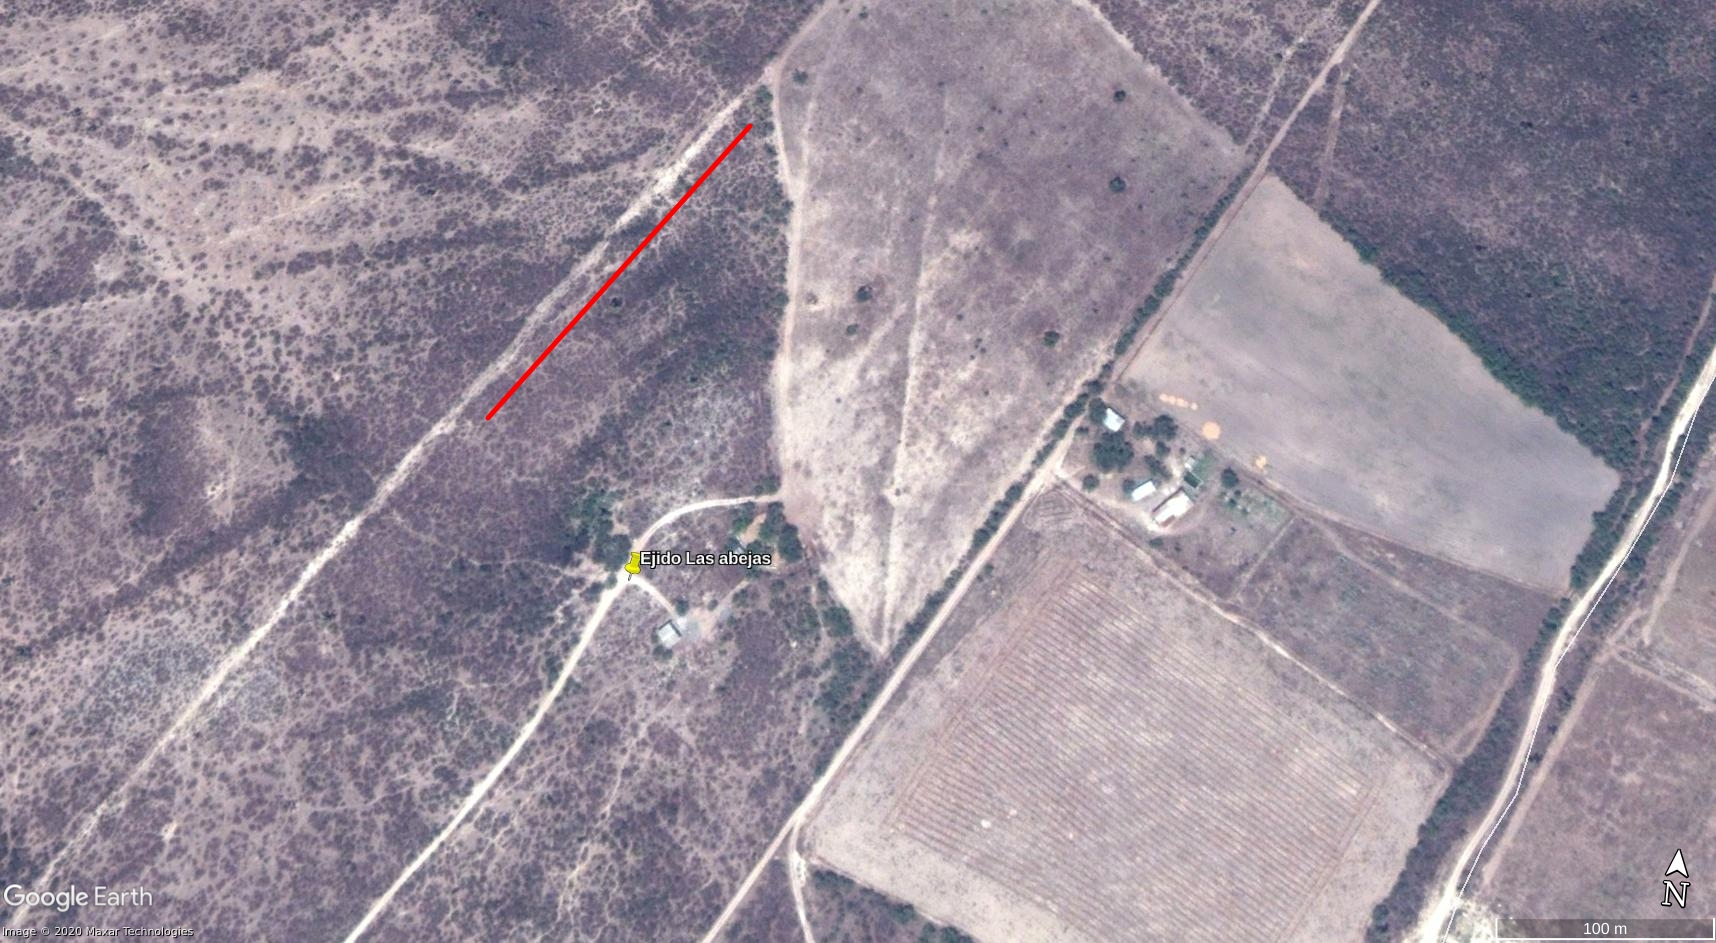
\includegraphics[scale=0.155]{110518r.jpg}
            \caption{Día 18/May/2011: aparece el camino}
        \end{subfigure}
        \begin{subfigure}{3.5\textwidth}
            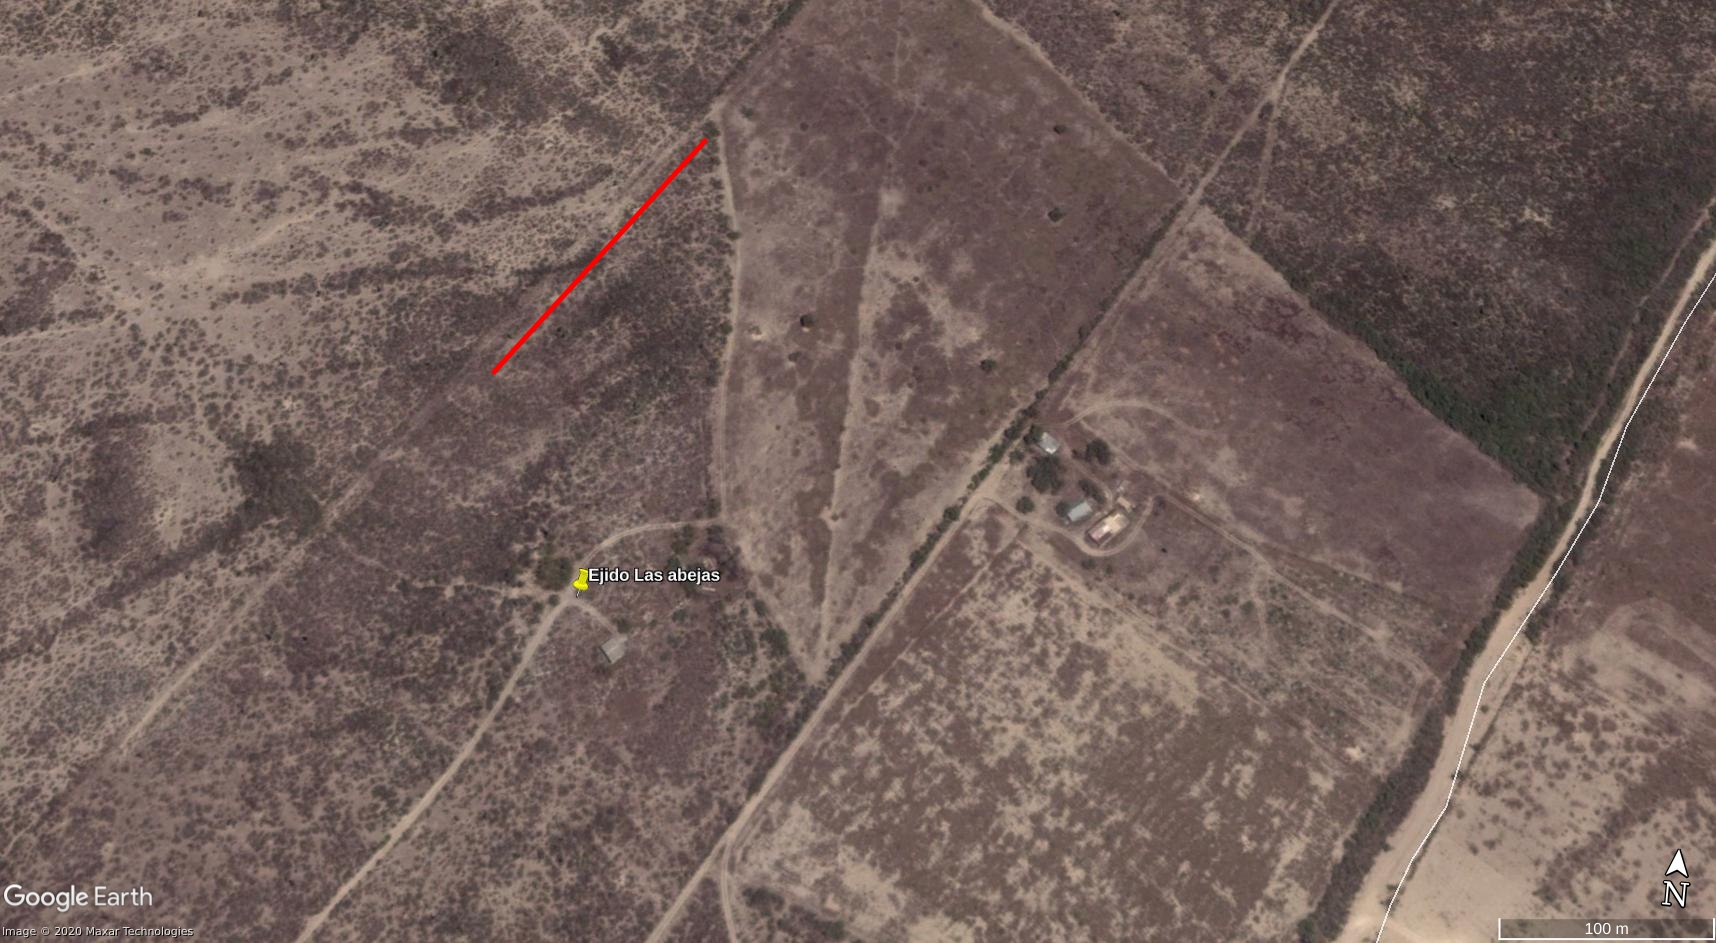
\includegraphics[scale=0.155]{140817r.jpg}
            \caption{Día 04/Mar/2016: se desvanece}
        \end{subfigure}
        \begin{subfigure}{3.5\textwidth}
            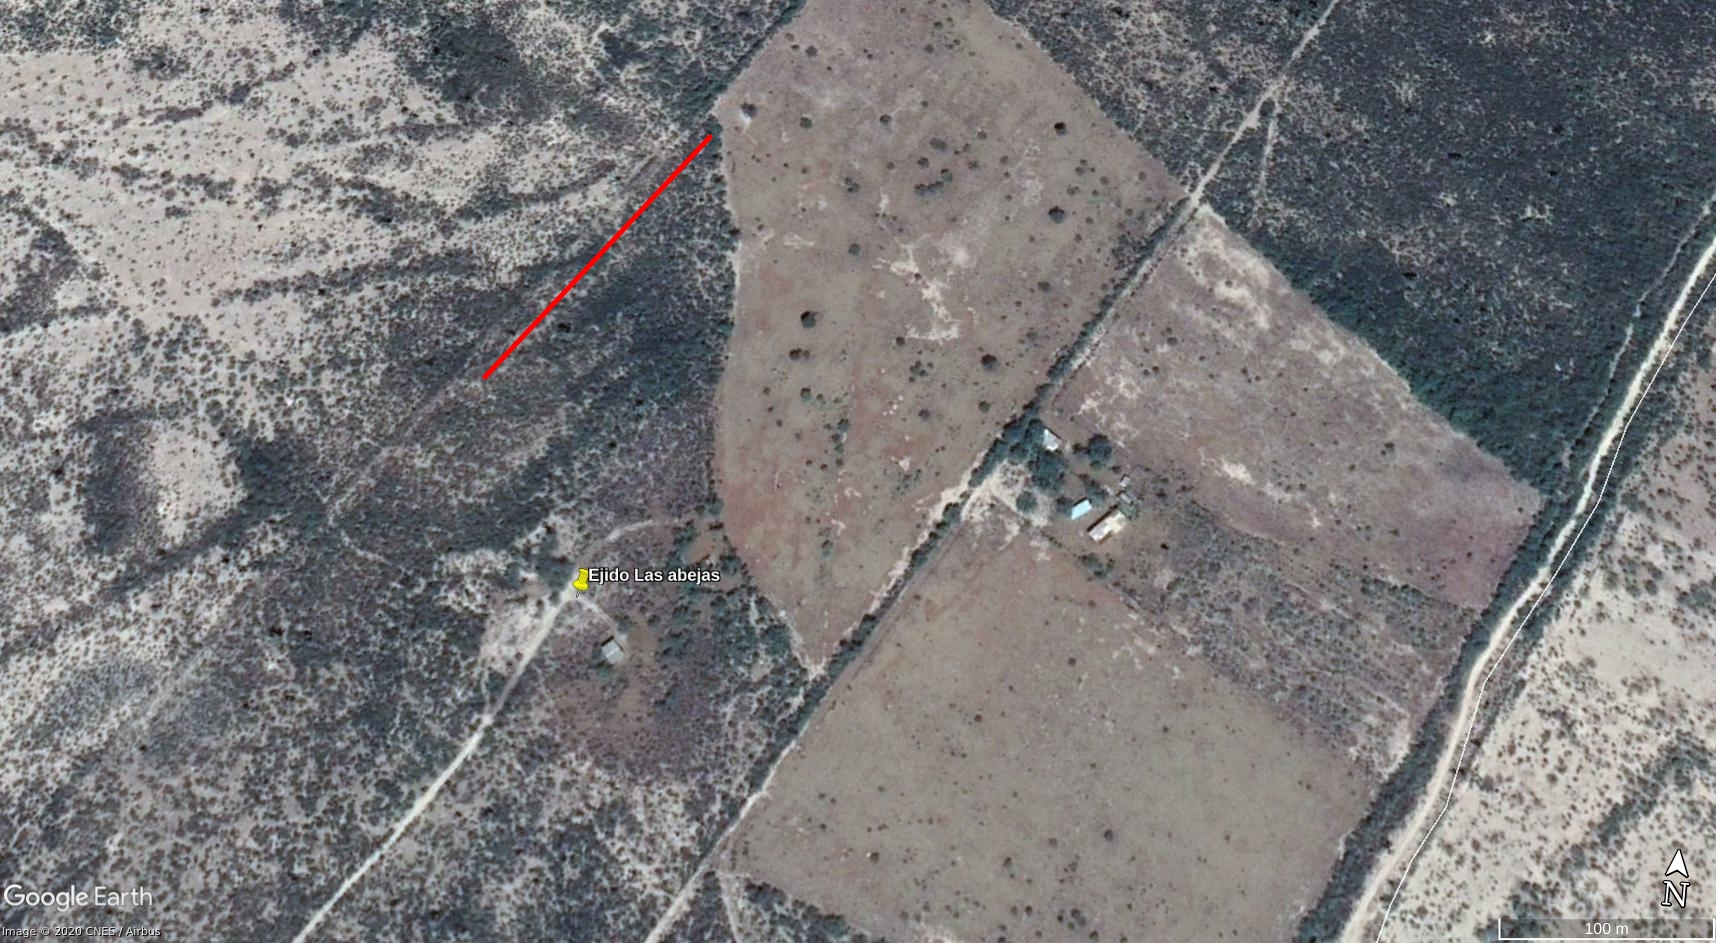
\includegraphics[scale=0.155]{190810r.jpg}
            \caption{Día 19/Ago/2019: casi imperceptible}
        \end{subfigure}
        \caption{Ejido "Las Abejas" (marcador amarillo): Línea roja señala al costado izquierdo el camino creado entre el (a) May/2007 y el (b) May/2011. Después entre Mar/2016 (c) y  Ago/2019(d) se ve el desvanecimiento.}
    \end{figure}
    \pagebreak
    \item Entre 14/May/2017 y 10/Ago/2019, se ve un incremento en la desertificación frente de la casa/almacén.
    \begin{figure}[H]
        \centering
        \begin{subfigure}{5\textwidth}
            \centering
            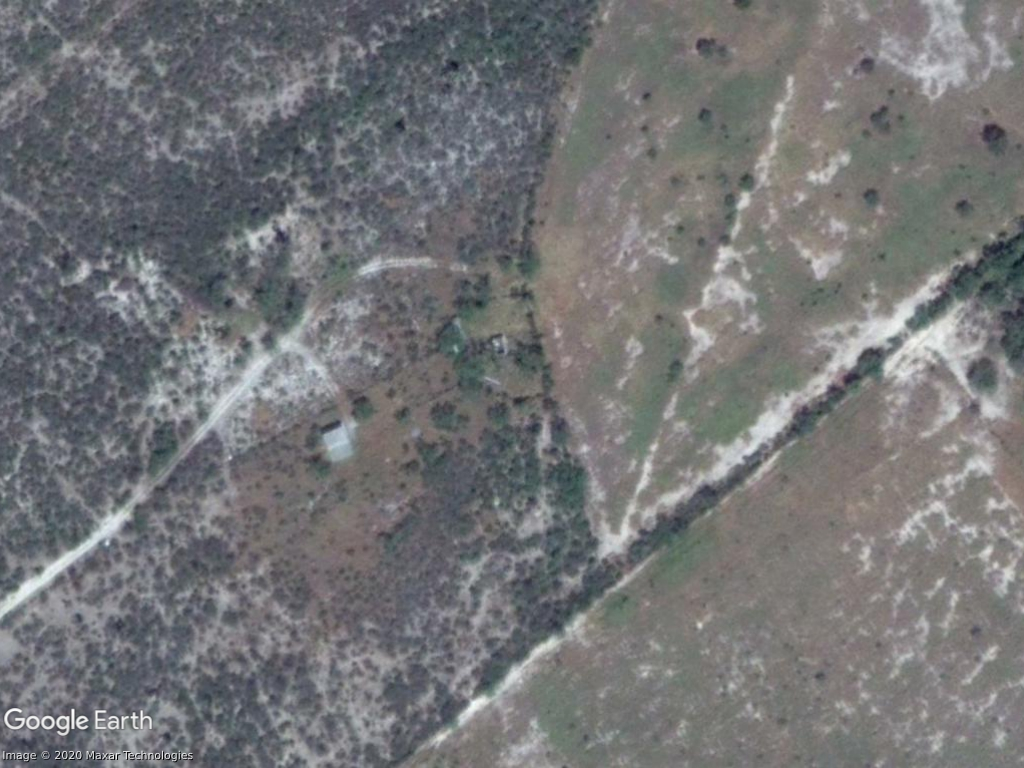
\includegraphics[scale=0.45]{region_1/20170514.jpg}
            \caption{Día 14/May/2017.}
        \end{subfigure}\\
        \begin{subfigure}{5\textwidth}
            \centering
            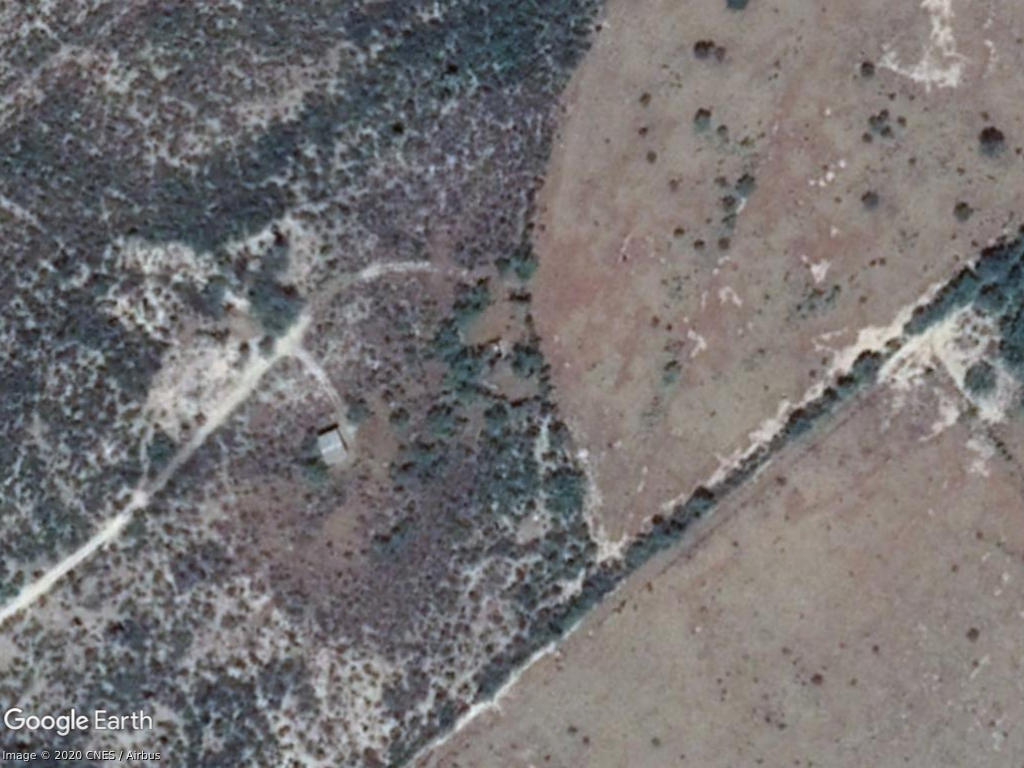
\includegraphics[scale=0.45]{region_1/20190810.jpg}
            \caption{Día 10/Ago/2019.}
        \end{subfigure}
        \caption{Aumento del área de terracería (tierra blanca) frente a la casa/almacén.}
    \end{figure}
    \pagebreak
    \item Entre el 22/May/2007 (\autoref{fig:caminos1}) y el 18/May/2011 (\autoref{fig:caminos2}) se desmontaron arbustos y aparecieron grietas cerca de éstos. 
    \begin{figure}[H]
        \centering
        \begin{subfigure}{5\textwidth}
            \centering
            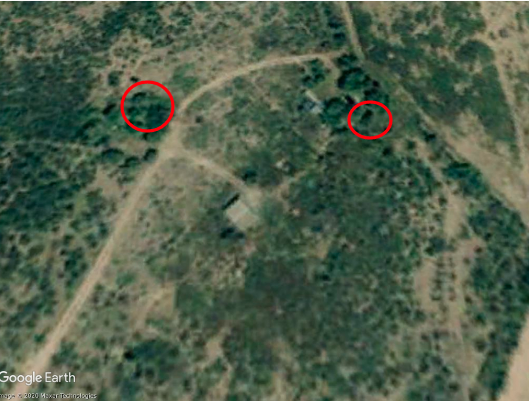
\includegraphics[scale=0.6]{figure3.png}
            \caption{Día 22/May/2007: Áreas verdes que cambiaron años más tarde, identificadas en círculos rojos.}
            \label{fig:caminos1}
        \end{subfigure}\\
        \begin{subfigure}{5\textwidth}
            \centering
            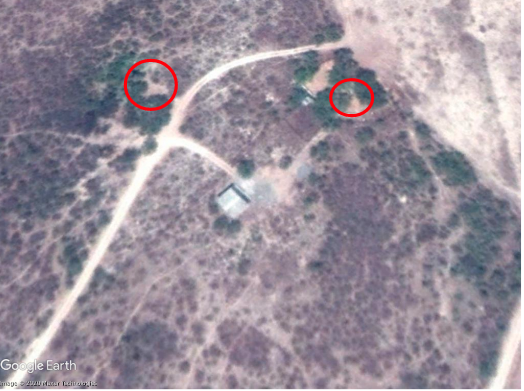
\includegraphics[scale=0.6]{figure4.png}
            \caption{Día 18/May/2011: Pérdida de cobertura de árboles y aparición de grietas.}
            \label{fig:caminos2}
        \end{subfigure}
        \caption{Zonas pequeñas donde cambió la cobertura de arbustos.}
        \label{fig:caminos_2007}
    \end{figure}
    \pagebreak
    \item La imagen del 20/Nov/2011 se toma como referencia de la cobertura de árboles cerca del predio, en la zona superior derecha. En la secuencia de imágenes desde Jun/2013 (b) pasando por Ago/2015 (c) va disminuyendo hasta llegar a un mínimo en el día 04/Abr/2016, donde a la fecha sigue igual.
    \begin{figure}[H]
        \begin{subfigure}{3.5\textwidth}
            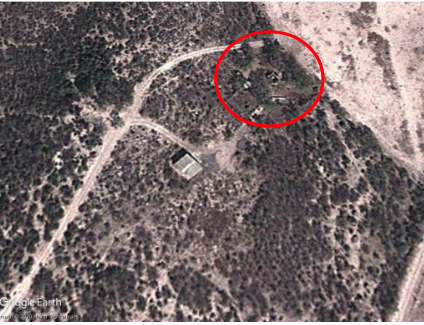
\includegraphics[scale=0.42]{20111120.png}
            \caption{Día 20/Nov/2011: Referencia de área verde.}
        \end{subfigure}
        \begin{subfigure}{3.5\textwidth}
            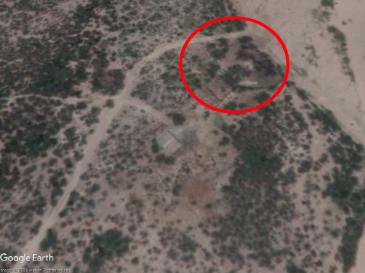
\includegraphics[scale=0.48]{20130606.png}
            \caption{Día 06/Jun/2013: Se redujo el área verde y se abrió un camino para ingresar al predio.}
        \end{subfigure}
        \begin{subfigure}{3.5\textwidth}
            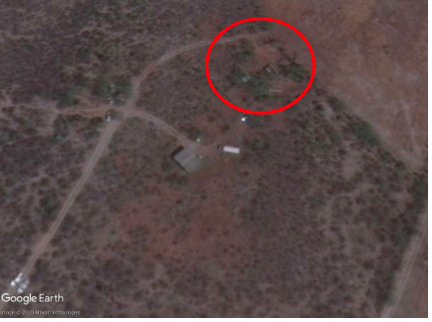
\includegraphics[scale=0.42]{20150812.png}
            \caption{Día 12/Ago/2015: El área árida es mayor.}
        \end{subfigure}
        \begin{subfigure}{3.5\textwidth}
            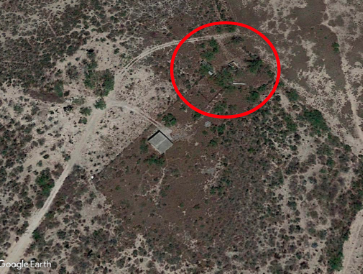
\includegraphics[scale=0.48]{20160404.png}
            \caption{Día 04/Abr/2016: Esta es la fecha donde se aprecian menos árboles.}
        \end{subfigure}
        \caption{Disminución del área verde.}
    \end{figure}
    \pagebreak
    \item En las imágenes previas al 17/Ago/2014 (\autoref{fig:arboles1}) se aprecia una distribución cercano a lo que podría ser un corral o pozo. Esta estructura tiene forma cuadrada. El 12/Ago/2015 (\autoref{fig:arboles2}) estos arbustos ya no aparecen.
    \begin{figure}[H]
        \centering
        \begin{subfigure}{5\textwidth}
        \centering
        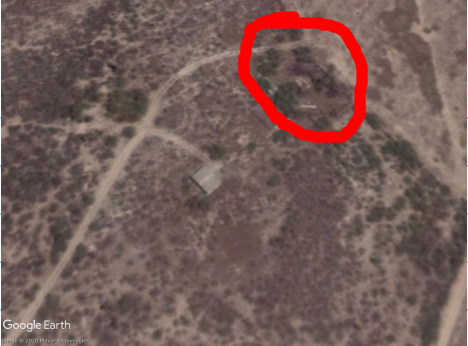
\includegraphics[scale=0.6]{figure1.png}
        \caption{Día 17/Ago/2014}
        \label{fig:arboles1}
        \end{subfigure}\\
        \begin{subfigure}{5\textwidth}
            \centering
            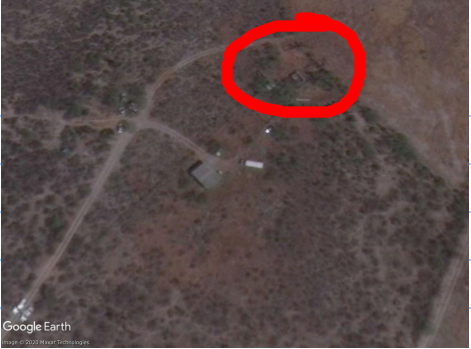
\includegraphics[scale=0.6]{figure2.png}
            \caption{Día 12/Ago/2015}
            \label{fig:arboles2}
            \end{subfigure}
        \caption{Los círculos rojos muestran la zona donde había arbustos (a) y posteriormente se registra (b) la pérdida de ellos entre 2014-2015.}
        \label{fig:arboles}
    \end{figure}
    \pagebreak
    \item El mismo 12/Ago/2015 al ingresar por la ruta principal se ven dos camionetas blancas bloqueando el camino. Más adelante cerca del cruce se distingue un posible grupo de vehículos de menor tamaño. Dentro del predio, al fondo, también se localiza una estructura blanca y larga, que podría ser una caja de tráiler (\autoref{fig:vehiculos}). El punto brillante que se ubica cerca de la caja de tráiler parece un objeto nuevo.
    \begin{figure}[H]
        \centering
        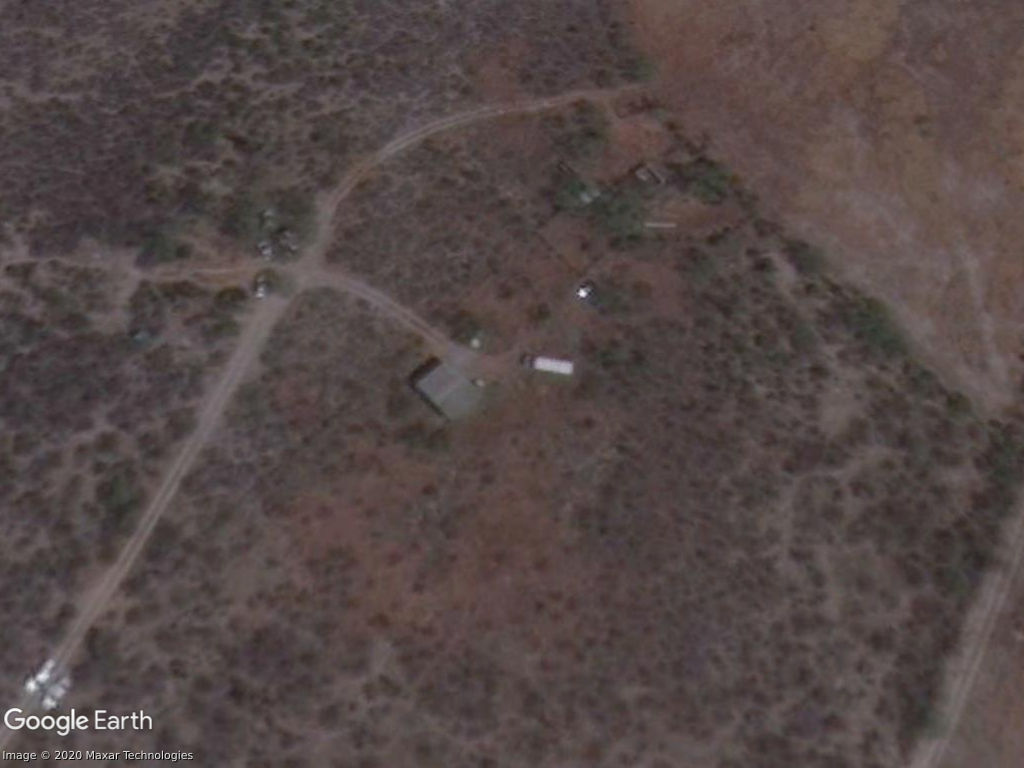
\includegraphics[scale=0.5]{region_2/20150812.jpg}
        \caption{Visualización de vehículos en la zona.}
        \label{fig:vehiculos}
    \end{figure}
    \pagebreak
    \item El día 28/Sep/2015 se visualiza una camioneta negra (\autoref{fig:camioneta_negra}) en la ruta principal (en la misma posición donde se encontraban las dos camionetas blancas el día 12/Agosto/2015). (\autoref{fig:vehiculos})
    \begin{figure}[H]
        \centering
        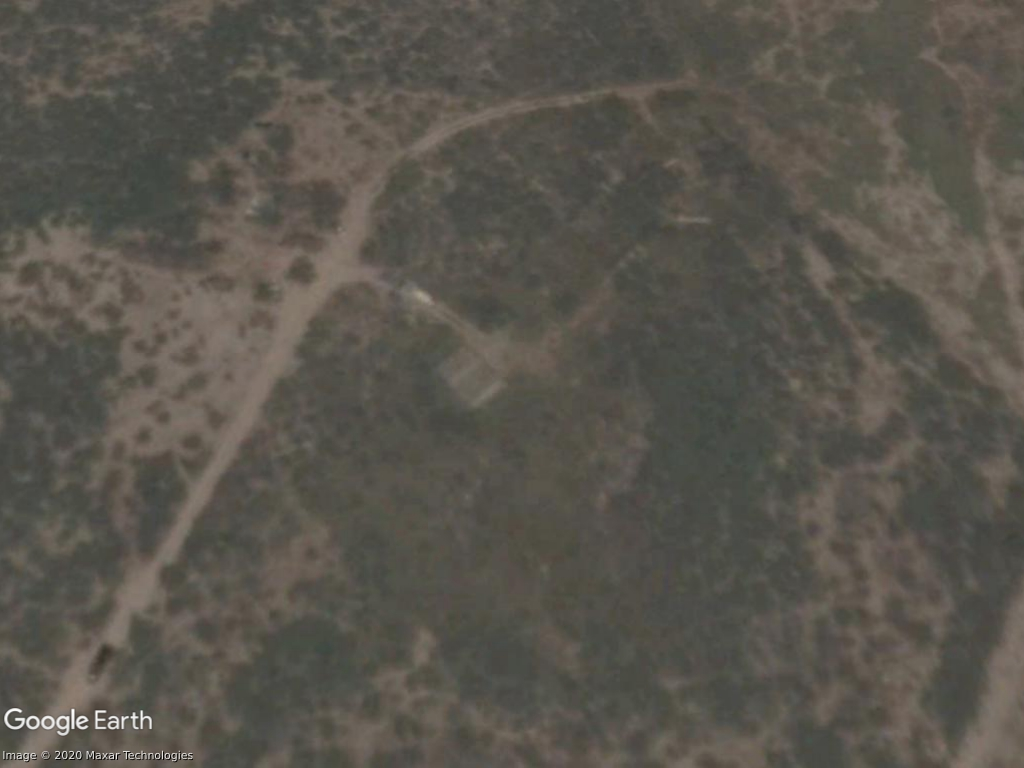
\includegraphics[scale=0.5]{region_2/20150928.jpg}
        \caption{Camioneta negra obstruyendo la ruta el día 28/Sep/2015.}
        \label{fig:camioneta_negra}
    \end{figure}
\end{enumerate}
Dra. Adriana Ipiña\\
Instituto de Física Rosario (CONICET-UNR), Rosario, Argentina\\
\\
Giovanni Gamaliel López-Padilla\\
Facultad de Ciencias Físico-Matemáticas, UANL, Monterrey, México


\end{document}

